\chapter{FUNDAMENTOS TEÓRICOS}
\section{Introducción} % {{{
El estudio de los sistemas cuánticos cerrados, es decir sistemas que no
interactúan con su entorno, nos ha permitido entender bastante bien muchos
fenómenos cuánticos. No obstante, una descripción más precisa 
requiere de considerar que los sistemas cuánticos reales son sistemas abiertos
que interactúan con su entorno. Para estudiar los 
sistemas cuánticos abiertos será útil revisar un formalismo distinto
al del vector de estado para describir a los estados cuánticos. 
Este formalismo es el de la matriz de densidad y tiene la ventaja 
de describir de manera más apropiada a los estados mixtos. 
Para la descripción de la evolución dinámica  
vamos a estudiar la teoría de los canales cuánticos, 
que es un marco teórico en el cual se considera que los estados 
cuánticos (matriz de densidad) evolucionan de forma discreta.

La estructura de este capítulo es la siguiente.
En la sección \ref{sec:ensambles} revisaremos una motivación para introducir 
a la matriz de densidad a partir de un ensamble de estados. 
Seguidamente, en la sección \ref{sec:density-matrices-properties},
estudiaremos las propiedades que debe cumplir una matriz 
de densidad para representar un estado cuántico
y cómo se reformulan los postulados 
de la mecánica cuántica utilizando este nuevo formalismo.
En la sección \ref{sec:qtm-channels} vamos a revisar las
condiciones para que un canal cuántico describa la evolución 
física de la matriz de densida. Por último, en la sección
\ref{sec:qtm-channels-representation}, vamos a estudiar 
la representación de superoperador y de Kraus de un canal cuántico.

% }}}
\section{Ensambles de estados cuánticos} \label{sec:ensambles} % {{{
% \esqueleto{Un copy-paste de la sección 1.1 del informe final de 
% prácticas. Voy a retocar alguna parte si fuera necesario, como ser
% más formal o agregar alguna prueba.}

Para introducir la definición de la matriz de densidad presentamos la 
motivación que exponen Sakurai y Napolitano \cite{sakurai_napolitano_2017}.
Consideremos un sistema cuántico que se encuentra en alguno de los estados 
$\Pk{i}$ con probabilidad $p_i$. Esto induce naturalmente el 
ensamble de estados del sistema $\{p_i, \ket{\psi_i} \}$. 
Supongamos que realizamos 
la medición de algún observable $\Lambda$ sobre el ensamble. El 
valor esperado al medir $\Lambda$ sobre este sistema es
\begin{align}\label{eq:expVal-expanded-Lambda}
	\expval{\Lambda} &= \sum_i p_i \matrixel{\psii}{\Lambda}{\psii}
	= \sum_{i,j,k} p_i 
	\bra{\psii}\dyad{\phi_j}{\phi_j}\Lambda\dyad{\phi_k}{\phi_k}\Pk{i},
\end{align}
con $\ket{\phi_j}$ es una base ortonormal del
espacio de Hilbert del sistema. Si se reordena
\eqref{eq:expVal-expanded-Lambda} de manera apropiada
se obtiene una expresión 
que motiva claramente la definición de la matriz de densidad $\rho$,
\begin{align}\label{eq:expVa-Lambda-wRho}
	\expval{\Lambda}&= \sum _{j,k}\bra{\phi_k}\qty(\sum_ip_i \dyad{\psii}{\psii} 
	)\ket{\phi_j}	\matrixel{\phi_j}{\Lambda}{\phi_k}.
\end{align}
La matriz que se encuentra entre paréntesis se define como 
la matriz de densidad 
$\rho$~\cite{nielsen_chuang_2011, sakurai_napolitano_2017}
\begin{equation}\label{eq:rho_def}
	\rho \equiv \sum _i p_i\dyad{\psi_i}{\psi_i}.
\end{equation}
Notemos que un elemento de matriz de $\rho$, escrita en la base 
$\ket{\phi_j}$, es
\begin{align}
	\matrixel{\phi_k}{\rho}{\phi_j} = 
	\sum_ip_i \braket{\phi_k}{\psii}\braket{\psii}{\phi_j},
\end{align}
por lo tanto, sustituyendo en la ecuación \eqref{eq:expVa-Lambda-wRho}
se tiene que el valor promedio del observable $\Lambda$ es
\begin{align}\label{eq:Tr(rhoLambda)}
	\expval{\Lambda}=\sum _k \matrixel{\phi_k}{\rho \Lambda}{\phi_k} 
	= \Tr \qty(\rho\Lambda).
\end{align} 
%Este resultado muestra cómo a partir de la matriz de densidad $\rho$ 
%se puede calcular toda la información física disponible de un sistema al 
%realizar una medición. 
Este resultado es interesante porque muestra que es posible 
calcular el valor promedio de un observable utilizando la 
matriz de densidad del sistema. En virtud de este resultado
vale la pena investigar a continuación cómo evoluciona la 
matriz de densidad de un sistema.
%Desde luego la matriz de densidad es una herramienta con la que
%se puede formular matemáticamente la mecánica cuántica como 
%con el vector de estado.
% \cpnote{Esta frase la pondría
% al principio del capítulo y lo que sigue del párrafo lo pondría al mismo 
% nivel conceptual que la discusión anterior. }. 
% \janote{De acuerdo. En la última iteración que hice de la introducción
% tome en cuenta este comentario tuyo.}
% 
% \janote{Me habías dejado los siguientes dos comentarios entre el texto
% que tenía antes. Así que opté por reescribir el desarrollo de la evolución
% dinámica de una vez con el operador $U$.}
% \cpnote{En aras de la simplicidad, 
% yo formularía el ejemplo directamente con al $U$. No hay necesidad de traer el 
% Hamiltoniano acá.}
% \cpnote{El título 
% de la siguiente sección contradice la ultima frase. quizá vale la pena que revises
% este caputulo y lo leas todo a ver si hay mas problemas como de estructura. }
% 

Consideremos un sistema que se encuentra en el ensamble 
de estados inicial $\{ p_i, \ket{\psi_i(0)}\}$
y que evoluciona según algún operador unitario $U(t)$. Es decir, 
el ensamble de estados en cualquier tiempo $t>0$ está dado por 
$\{p_i, U(t)\ket{\psi_i(0)}\}$. Entonces, utilizando la definición 
\eqref{eq:rho_def} recién introducida, la matriz de
densidad $\rho(t)$ del sistema será
\begin{align} \label{eq:Rho-evolution-H}
	\rho(t) &= \sum_i p_i\dyad{\psi_i(t)}{\psi_i(t)}\nonumber\\
	&= \sum_i p_i U(t) \dyad{\psi_i(0)}{\psi_i(0)}U^{\dagger}(t)
	\nonumber\\
	&= U(t)\rho(0)U^{\dagger}(t),
\end{align}
donde $\rho(0)$ es la matriz de densidad del ensamble 
de estados inicial $\{p_i, \ket{\psii(0)}\}$. Hemos probado así
que la descripción dinámica de un sistema que evoluciona 
según un operador unitario puede hacerse utilizando 
su matriz de densidad. En la sección que sigue 
estudiaremos las propiedades que deben satisfacer 
las matrices de densidad en general y revisaremos cómo 
formular los postulados de la mecánica cuántica con la matriz de densidad.

%
%Por ejemplo, veamos a continuación cómo 
%describir la evolución de un sistema cuántico cerrado.
%Consideremos un sistema cuyo Hamiltoniano es $H$, y es
%independiente del tiempo. Bajo estas condiciones la evolución
%del sistema está descrita por 
%$\ket{\psi (t)}=U(t)\ket{\psi(0)}$~\cite{sakurai2010modern}. 
%Sin embargo, consideremos que el sistema se encuentra inicialmente
%en un ensamble de estados $\{p_i, \ket{\psii(0)}\}$, por lo cual
%el estado final del sistema será 
%$\{p_i, \ket{\psii(t)}\}$.
%Por consiguiente, el matriz de densidad final $\rho(t)$  es 
%\begin{align} \label{eq:Rho-evolution-H}
%	\rho(t) &= \sum_j p_j\dyad{\psi_j(t)}{\psi_j(t)}\nonumber\\
%	&= \sum_j p_j U(t) \dyad{\psi_j(0)}{\psi_j(0)}U^{\dagger}(t)
%	\nonumber\\
%	&= e^{-iHt}\rho(0)e^{iHt},
%\end{align}
%donde $\rho(0)$ es la matriz de densidad que describe al ensamble 
%de estados inicial $\{p_i, \ket{\psii(0)}\}$.	 Aunque hemos desarrollado 
%un ejemplo para la evolución de un sistema cuyo Hamiltoniano es 
%independiente del tiempo, es sencillo de ver que en general la dinámica  
%de un sistema cerrado se describe como 
%\begin{align}\label{eq:rho-ClosedEvolution}
%\rho(0) \longrightarrow U\rho(0)U^{\dagger}.
%\end{align}
%Con esto, se ha asegurado que la dinámica de un sistema cuántico puede 
%describirse utilizando su matriz de densidad. 


%Las ecuaciones \eqref{eq:Tr(rhoLambda)} y \eqref{eq:rho-ClosedEvolution}
%muestran que la matriz de densidad puede utilizarse para la descripción 
%de la medición y la evolución de los estados cuánticos. 
%En la siguiente sección veremos la formulación de los postulados 
%de la mecánica cuántica utilizando la matriz de densidad. 


% }}}
\section{Propiedades de la matriz de densidad} % {{{
% \cpnote{Aca voy. Lo anterior ya queda listo}
\label{sec:density-matrices-properties}
% \esqueleto{Revisando esta sección en el informe de prácticas 
% veo que me gustaría ir aquí más al grano y mandar al lector 
% a las pruebas en el Chuang (para no copiar otra vez las pruebas
% aquí). Puntualizaré: (1) caracterización de la matriz de densidad, (2)
% postulados de la mecánica cuántica usando la matriz de densidad y
% (3) matriz de densidad reducida.}


A pesar de que contamos con la definición \eqref{eq:rho_def} de 
la matriz de densidad dado un ensamble de estados, será útil 
estudiar cuáles son las condiciones que una matriz debe cumplir 
para ser una matriz de densidad. Luego de esto, estamos listos 
para revisar la formulación de los postulados de la mecánica cuántica
utilizando la matriz de densidad. Por último, vamos a estudiar la
matriz de densidad reducida, la manera para describir a los
subsistemas de sistemas compuestos con el formalismo 
de la matriz de densidad.
% \cpnote{La matriz de densidad es una
% matriz, no una aplicación (en su manera más simple\ldots). Quizá te 
% quieras referir a la traza parcial?}\janote{No. Me refiero a una 
% aplicación del formalismo de la matriz de densidad. Reformulé 
% esa frase.}

Las propiedades que una matriz debe tener para que esta represente al 
estado físico de un sistema se establecen a continuación
\cite{nielsen_chuang_2011}:
\begin{thm}\label{teo:density-operator}
Una matriz $\rho$  que actúa sobre el espacio de Hilbert de un sistema 
es la matriz de densidad asociada a algún ensamble 
$\{p_i, \ket{\psi _i} \}$ si y sólo si satisface las condiciones:
\begin{enumerate}
\item $\Tr \rho = 1$.
\item $\matrixel{\psi}{\rho}{\psi} \geq 0$, $\forall\ket{\psi} \in \hi$.
\end{enumerate}	
\end{thm} 
\begin{proof} Consultar~\cite[p.~101]{nielsen_chuang_2011} \end{proof}

La condición de traza unitaria de la matriz de densidad es análoga
a la condición de normalización de la función de onda, las probabilidades
de medir al sistema en un estado u otro deben sumar uno. 
Por otro lado, los eigenvalores $\lambda_i$ y eigenvectores $\ket{\psi_i}$ de la 
matriz de densidad definen a uno de los posibles ensambles de estados
$\{\lambda_i, \ket{\psi_i} \}$ del sistema. Entonces,
la condición de positividad de la matriz de densidad asegura que las
probabilidades $\lambda_i$ de encontrar al sistema en el estado $\ket{\psi_i}$
son cero o positivas, como esperaríamos que fuese. 
% \cpnote{Siengo que la notación
% $A\ge 0$ no es obvia. Quizá quieras decir en este párrafo que es. Lo dices 
% implicitamente, pero creo qe hay que ser tantito mas explicito.}\janote{Qué
% tal mejor sólo modificar la notación para la positividad en el teorema 1.3.1
% así como lo hice?}

Ahora que que ya contamos con una definición de la matriz de densidad 
que no parte de conocer \textit{apriori} el ensamble de estados del sistema
nos ocupamos de la formulación de los postulados de la mecánica cuántica 
utilizando este nuevo formalismo~\cite[p.~102]{nielsen_chuang_2011}.
\begin{itemize}
	\item[] \textbf{Postulado 1.} \textit{Estado del sistema.} 
	Un sistema físico tiene asociado un espacio vectorial complejo
	con producto interno conocido como el espacio de Hilbert $\hi$ del
	sistema. Los estados del sistema están descritos por el conjunto 
	de matrices de densidad que actúan sobre $\hi$.
	\item[] \textbf{Postulado 2.} \textit{Evolución unitaria.}
	La evolución de un sistema cuántico cerrado, en un intervalo 
	de tiempo $[t_1,t_2]$, está descrita	por una transformación unitaria $U$
	de la siguiente manera 
	\begin{equation} \label{eq:postulate-ClosedEvolution}
	\rho(t_1)\longrightarrow U\rho(t_1) U^{\dagger}=\rho(t_2).
	\end{equation}
	\item[] \textbf{Postulado 3.} \textit{Medición.}
	Las mediciones sobre el estado $\rho$ de un sistema 
	están descritas por un conjunto de operadores $\{M_m\}$. 
	Estos son operadores que actúan sobre $\hi$ y el 
	índice $m$ refiere a los posibles
	resultados de la medición. Si el estado del sistema es $\rho$ 
	inmediatamente antes de la medición, entonces la probabilidad
	$p(m)$ de obtener el resultado $m$ es
	\begin{equation} \label{eq:post_MeasureProb}
	p(m)=\Tr \qty(M_m^{\dagger}M_m\rho),
	\end{equation}						
	y el estado del sistema inmediatamente después de la medición será
	\begin{equation} \label{eq:post_MeasureTrasnfState}
	\rho'=\frac{M_m\rho M_m^{\dagger}}{\tr \qty(M_m^{\dagger}M_m\rho)}.
	\end{equation}	
	Los operadores $M_m$ deben satisfacer la ecuación de completitud
	\begin{equation} \label{eq:post_MeasureMCompleteness}
	\sum _m M_m^{\dagger}M_m=\mathbb{1}.
	\end{equation}
	\item[] \textbf{Postulado 4.} \textit{Sistemas de partículas.}
	El espacio de Hilbert de un sistema 	de varias partículas se compone del
	producto tensorial de los espacios de Hilbert 	individuales.
	Es decir, si el sistema total se compone de $N$ partículas, 
	entonces el espacio de Hilbert total es
	\begin{align}\label{eq:postulado4}
		\hi_{\txt{total}} = \hi_1\ten \hi_2 \ten \ldots \ten \hi_N.
	\end{align}
	Los estados del sistema total están descritos por las matrices de 
	densidad que actúan sobre $\hi _{\text{total}}$.
\end{itemize}

% Respecto al último postulado debemos resaltar que no todos 
% los estados del sistema total son de la forma $\rho=\rho_1
% \ot \ldots \ot \rho_N$. Es decir, no todos los estados del sistema 
% total son factorizables \cpnote{Acá tenemos que hablar. Hay varios tipos de estados, 
% los factorizables, los separables y los enlazados. Siento que no conoces la diferencia 
% entre los primeros dos. Hablamos y corriges este parrafo por favor}
% \janote{Ve directo al siguiente comentario}, pues el
% conjunto de los estados del sistema total también está compuesto por estados 
% no factorizables, también llamados entrelazados.
% Son justo los estados entrelazados los que conducen a hacernos preguntas
% como ¿cuál es el estado en el que se encuentra sólo una parte del sistema total?
% Seremos más claros con un ejemplo. Si un sistema bipartito 
% se encuentra en un estado factorizable $\rho\ot \sigma$ sabemos 
% que una parte del sistema se encuentra en el estado $\rho$ y la otra 
% en el estado $\sigma$. No obstante, ¿cuál es el estado
% de bipartición del sistema cuando el estado total es uno entrelazado
% ($\rho_{\text{total}}\neq\rho\ot \sigma$)? O,
% al menos, es deseable conocer cuál es la información accesible 
% para un observable de sólo una parte del sistema. Para responder a 
% estas preguntas revisaremos en lo que resta de esta sección
% la matriz de densidad reducida. Esta aplicación de la matriz de densidad 
% proporciona una herramienta para la descripción de subsistemas 
% de sistemas cuánticos compuestos~\cite{nielsen_chuang_2011}.
% \cpnote{Creo que igual este párrafo sobra. De nuevo, lo platicamos}
% \janote{Quisiera mantenerlo porque hace una transición de hablar 
% de los postulados a la matriz de densidad reducida. Lo iteré y es 
% el párrafo nuevo que le sigue a este comentario:}

Debemos resaltar que aunque el espacio de Hilbert de muchas partículas 
es de la forma \eqref{eq:postulado4} no todas las matrices de densidad
que actúan sobre son de la forma 
\begin{align}
\rho_{\text{total}}=\rho_1\ot \rho_2\ot \ldots\ot \rho_n,
\end{align}
lo cual nos conduce a preguntarnos que dada una matriz de densidad de
un sistema compuesto $\rho_{\text{total}}$, ¿cuál es el estado 
en el que se encuentra cada uno de los subsistemas que lo componen?
Por esta razón, para averiguar cómo describir a los subsistemas con 
el formalismo de la matriz de densidad es que vamos a revisar a continuación
cómo introducir la matriz de densidad reducida utilizando una herramienta
conocida como la traza parcial \cite{nielsen_chuang_2011}. 
% \janote{Si este párrafo te pareció bien habría que borrar el anterior.}



Supongamos dos subsistemas $A$ y $B$ cuyo estado total es 
$\rho^{AB}$ (en general $\rho^{AB}\neq \rho^A\ot \rho^B$). 
Consideremos una base ortonormal $\ket{\psi_i}$ de $\hi_A$ y una 
base ortonormal $\ket{\phi_j}$ de $\hi_B$. Una base ortonormal 
del sistema total $\hi_{\text{total}}$ está dado 
por $\ket{\psi_i}\ot \ket{\phi_j}$.
En esta base un elemento de matriz de $\rho^{AB}$ está dado por
\begin{align}
	\bra{\psi_i}\bra{\phi_j}\rho^{AB}\ket{\psi_k}\ket{\phi_l},
\end{align}
donde hemos utilizado la notación 
$\ket{\psi}\ot\ket{\phi}=\ket{\psi}\ket{\phi}$.
Supongamos que $\Omega_A\ot \1$ es un observable que actúa sobre $A$
en $\hi_{\text{total}}$ y el valor esperado 
$\expval{\Omega_A\ot \1}$, utilizando~\eqref{eq:Tr(rhoLambda)},~es
\begin{align}
	\Tr \qty(\rho^{AB}\qty(\Omega_A\ot \mathbb{1})) &= \sum _{i,j} 
	\bra{\psi_i}\bra{\phi_j}\rho^{AB}\qty(\Omega_A\ot \mathbb{1})
	\ket{\psi_i}\ket{\phi_j} 
	\nonumber\\
	&= \sum _{i,j} 
	\bra{\psi_i} \bra{\phi_j}\rho^{AB}
	\qty(\sum _{k,l} \ket{\psi_k} \ket{\phi_l} \bra{\psi_k}\bra{\phi_l} )
	\qty(\Omega_A\ot \mathbb{1})\ket{\psi_i} \ket{\phi_j}\nonumber\\
	&= \sum _{i,j,k,l} 
	\bra{\psi_i} \bra{\phi_j}\rho^{AB}\ket{\psi_k} \ket{\phi_l}
	\matrixel{\psi_k}{\Omega_A}{\psi_i}\delta _{lj}\nonumber\\
	&= \sum_{i,k}\qty(\sum _j 
	\bra{\psi_i} \bra{\phi_j}\rho^{AB}\ket{\psi_k} \ket{\phi_j})
	\matrixel{\psi_k}{\Omega_A}{\psi_i}.
	\label{eq:almost-reducedRho}
\end{align}
% donde hemos utilizado $\ket{\psi}\ot\ket{\phi}=\ket{\psi}\ket{\phi}$\cpnote{Esto
% es mas bien una definicipon que de hecho puedes hacer más arriba}
% \janote{Listo. Lo definí después de la ecuación 1.13. Si te parece bien 
% porfa lo que sigue aquí}.
La matriz entre paréntesis define a la matriz de densidad
reducida $\rho^A$ del subsistema $A$ como~\cite{chandra2013quantum}
\begin{align}
	\sum _j \bra{\psi_i}\bra{\phi_j}\rho^{AB}\ket{\psi_k}\ket{\phi_j}
	= \matrixel{\psi_i}{\rho^A}{\psi_k}.
	\label{eq:reducedRho-def1}
\end{align}
y retomando el cálculo de $\expval{\Omega_A\ot \1}$
en \eqref{eq:almost-reducedRho} se obtiene, en función de $\rho^A$,
\begin{align}
	\Tr \qty(\rho^{AB}\qty(\Omega_A\ot \mathbb{1}))&= \sum _{i,k}\nonumber
	\matrixel{\psi_i}{\rho^A}{\psi_k} \matrixel{\psi_k}{\Omega_A}{\psi_i}
	\nonumber\\
	&= \sum_i \matrixel{\psi_i}{\rho^A\Omega_A}{\psi_i}\nonumber\\
	&= \Tr \qty(\rho^A\Omega_A). \label{eq:reduced-works}
\end{align}
Notemos la similitud de este resultado con el que se obtuvo en la ecuación
\eqref{eq:Tr(rhoLambda)}. El valor esperado de un observable que actúa 
sobre sólo uno de los subsistemas puede calcularse con su matriz de 
densidad reducida.

Ya que mostramos la utilidad que puede tener la matriz de densidad
reducida, ahora vamos a discutir con detalle la operación que 
la define en \eqref{eq:reducedRho-def1}. 
Esta operación se conoce como traza parcial. El adjetivo `parcial'
es porque la operación de traza se realiza sólo sobre los grados 
de libertad de alguno de los subsistemas. En la ecuación 
\eqref{eq:reducedRho-def1} denotamos a la matriz de densidad 
reducida $\rho^A$ como la traza parcial sobre $B$ de $\rho^{AB}$,
\begin{align} 
	\sum _j \bra{\psi_i}\bra{\phi_j}\rho^{AB}\ket{\psi_k}\ket{\phi_j}
	&=\matrixel{\psi_i}{\Tr_B\qty(\rho^{AB})}{\psi_k}
	= \matrixel{\psi_i}{\rho^A}{\psi_k}.
	\label{eq:partialTrace-def}
\end{align}
En general, la traza parcial es una operación lineal
que se define como~\cite{nielsen_chuang_2011}
\begin{align}
	\Tr_B (\dyad{\alpha_i}{\alpha_j}\otimes \dyad{\beta_k}{\beta_l})
	\equiv
	\dyad{\alpha_i}{\alpha_j}\Tr \qty(\dyad{\beta_k}{\beta_l}),
	\label{eq:part_trace-def}
\end{align}
donde $\ket{\alpha_i}$ son vectores ortonormales del subespacio $\hi_A$
y $\ket{\beta_j}$ del resto del espacio de Hilbert total.\cpnote{Para que esta
definición esté completa, también tienes que decir que la traza parcial 
es lineal} \janote{De acuerdo. Hecho} \cpnote{Nel, aun no jala.} 
\janote{Ahora sí? Fíjate cómo modifiqué la línea 210.}

Ahora que contamos con las propiedades de la matriz de densidad, 
los postulados reescritos con este formalismo y la aplicación de la matriz
de densidad reducida para describir subsistemas ya disponemos de
las herramientas adecuadas para describir a los estados cuánticos 
utilizando a la matriz de densidad. En la siguiente sección continuamos 
con la evolución de la matriz de densidad utilizando la teoría de los 
canales cuánticos.

% }}}
\section{Canales cuánticos}\label{sec:qtm-channels} % {{{

La teoría de los canales cuánticos es un marco teórico con el cual 
se puede describir la evolución de los sistemas cuánticos abiertos.
Un canal cuántico es una operación lineal que debe preservar las 
propiedades de la matriz de densidad y que, cuando el sistema sea
parte de un sistema más grande junto con un \textit{ancilla}, la
extensión del canal que actúa sobre el sistema total debe también 
de preservar la traza y positividad de la matriz de densidad total.

% \cpnote{sobra lo de matrices de densidad. Si es abierto, vas a necesitar 
% una matriz de densidad, en general, se sobreentiende} \janote{Entendido}
%Un canal cuántico $\E$ es una operación lineal que transforma matrices
%de densidad en matrices de densidad y que es
%completamente positiva~\cite{bengtsson_zyczkowski_2017},
% \cpnote{Oye porque 
% tiene que ser afin? ME gustaría que me contaras mas en detalle} 
% \janote{Porque estaba confundiendo las cosas jeje. Está mal decir 
% que es un mapeo afín. Yo estaba asociando mal ser afín con mapear
% matrices de densidad en matrices de densidad. Revisé el GofQS y aclaré
% que un mapeo afín es otra cosa. Reformulé el enunciado anterior y posterior
% a este comentario donde utilizaba `mapeo afín'.}
%Un canal cuántico de preservar las propiedades de las matrices de densidad.
%Por otro lado, para entender qué es la completa positividad 
%y qué implica esto para la evolución dinámica de los estados 
%cuánticos vamos a elaborar en esta sección un ejemplo de 
%una operación que actúa sobre una partícula de espín 1/2 
%antes de definir formalmente la completa positividad.
Matemáticamente se escribe la acción de un canal cuántico $\E$ 
sobre un estado $\rho$ como
\begin{align} \label{eq:E(rho)}
\rho' = \E (\rho),
\end{align} 
donde $\E$ es una operación lineal y $\rho'$ es una matriz de
traza unitaria y positiva. Para que $\E$ sea un canal cuántico 
se requiere también que sea operación completamente positiva (CP). 
Antes de enunciar una de las definiciones de la completa positividad
vamos a elaborar un ejemplo con el objetivo de exponer mejor la 
implicación física de esta condición.

%Supongamos que vamos a estudiar 
%la dinámica de un sistema $P$, que hace parte de un sistema compuesto
%junto con un \textit{ancilla} $S$. Vamos a considerar que el 
%estado del \textit{ancilla} no lo conocemos \textit{a priori} o que 
%sencillamente no nos interesa. La condición de completa positividad
%sobre $\E$ se hace necesariar de imponer para que, aún cuando
%el sistema total se encuentre en un estado entrelazado,
%la extensión del canal cuántico que actúa sobre el 
%sistema compuesto preservará la positividad de 
%la matriz de densidad.
%\cpnote{Oye, la redaccion de este parrafo está horrible. Dale una iterada nueva, 
%descansado a la 1.4 por favor y me avisas}.

%\cpnote{Prometes que vas a dar un ejemplo antes, luego metes algo en la mitad
%y luego pones el ejemplo. Me parece un poco desordenado. Quizá puedes quitar
%la promesa anterior y acá explicar} \janote{Fue esto lo que empecé a 
%corregir y mejor terminé reescribiendo casi toda la sección.}

El ejemplo que vamos a discutir es el de una operación que actúa 
sobre $\rho$ como en \eqref{eq:E(rho)} \cpnote{no entiendo que quieres decir que
no satisfaga 1.19\ldots quizá quieres decir que mapea estados a estados? O como?} 
\janote{Sí, eso quiero decir. Modifiqué el enunciado, quedó mejor?}
pero que no es CP y, por consiguiente,
la extensión de la operación que actúa sobre un sistema que interactúa con un 
\textit{ancilla} no transforma al estado máximamente entrelazado en 
un estado físico. La operación que consideraremos 
actúa sobre partículas de espín 1/2, i.e. sistemas cuánticos de
dos niveles. En computación e información cuántica
se conoce a estos sistemas como qubits. Una manera
de escribir a la matriz de densidad de 1 qubit es
\begin{align}
\rho&=\frac{1}{2}\sum_{i=0}^{3} r_i\sigma_i,
\label{eq:rho-1qubit}
\end{align}
donde $\sigma_0=\1$ y el resto de $\sigma_i$ las 3 matrices de Pauli.
Imponemos que $r_0=1$ para que $\Tr(\rho)=1$.
Esta forma de escribir a la matriz de densidad de 1 qubit es útil porque
las componentes $r_1$, $r_2$ y $r_3$ especifican las coordenadas 
cartesianas de un punto en la esfera de Bloch, esfera unitaria que 
se utiliza para representar a los estados de 1 qubit. Similarmente, 
la matriz de densidad de 2 qubits se escribe como~\cite{nielsen_chuang_2011}
\begin{align}\label{eq:rho-2qubits}
\rho=\frac{1}{4}\sum _{i,j=0}^{3}r_{ij}\sigma_i\otimes\sigma_j,
\end{align}
con $r_{00}=1$.
Consideremos ahora la operación lineal $\E_z$ de 1 qubit
que mapea la esfera de Bloch a un disco sobre el plano $x$-$y$ 
como se muestra en la \Fref{fig:qtm-op-motivation}.
\cpnote{Creo que quitaste la figura}\janote{Listo. La agregué de nuevo.}
En términos de las componentes $r_i$, la operación $\E_z$ 
transforma a una matriz de densidad $\rho$ como en 
\eqref{eq:rho-1qubit} de la siguiente manera
\begin{align}
\qty(1,r_1,r_2,r_3)\mapsto\qty(1,r_1,r_2,0).
\end{align}
\begin{figure}% {{{
\centering
\begin{minipage}{.4\textwidth}
\centering
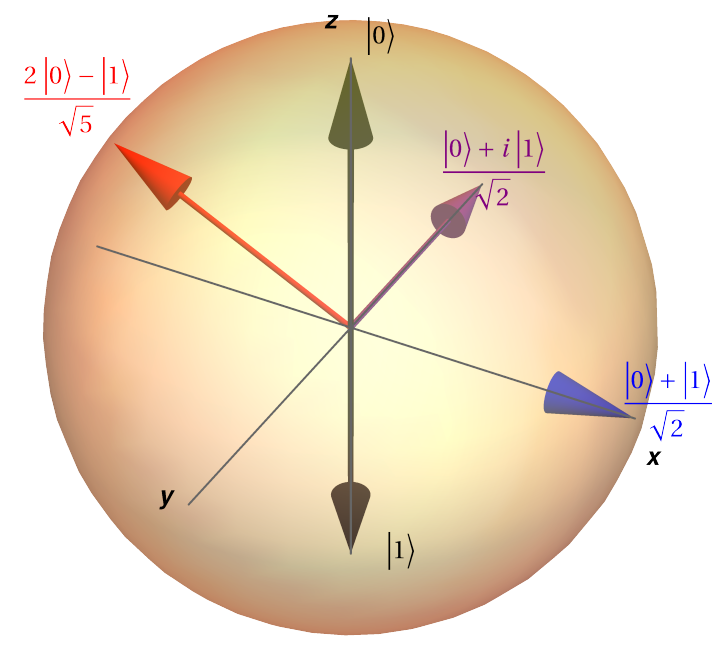
\includegraphics[width=5cm]{bloch.png}
\end{minipage}
$\stackrel{\E_{z}\otimes\1 \vspace{1cm}}{\longmapsto}$
\begin{minipage}{0.4\textwidth}
\centering
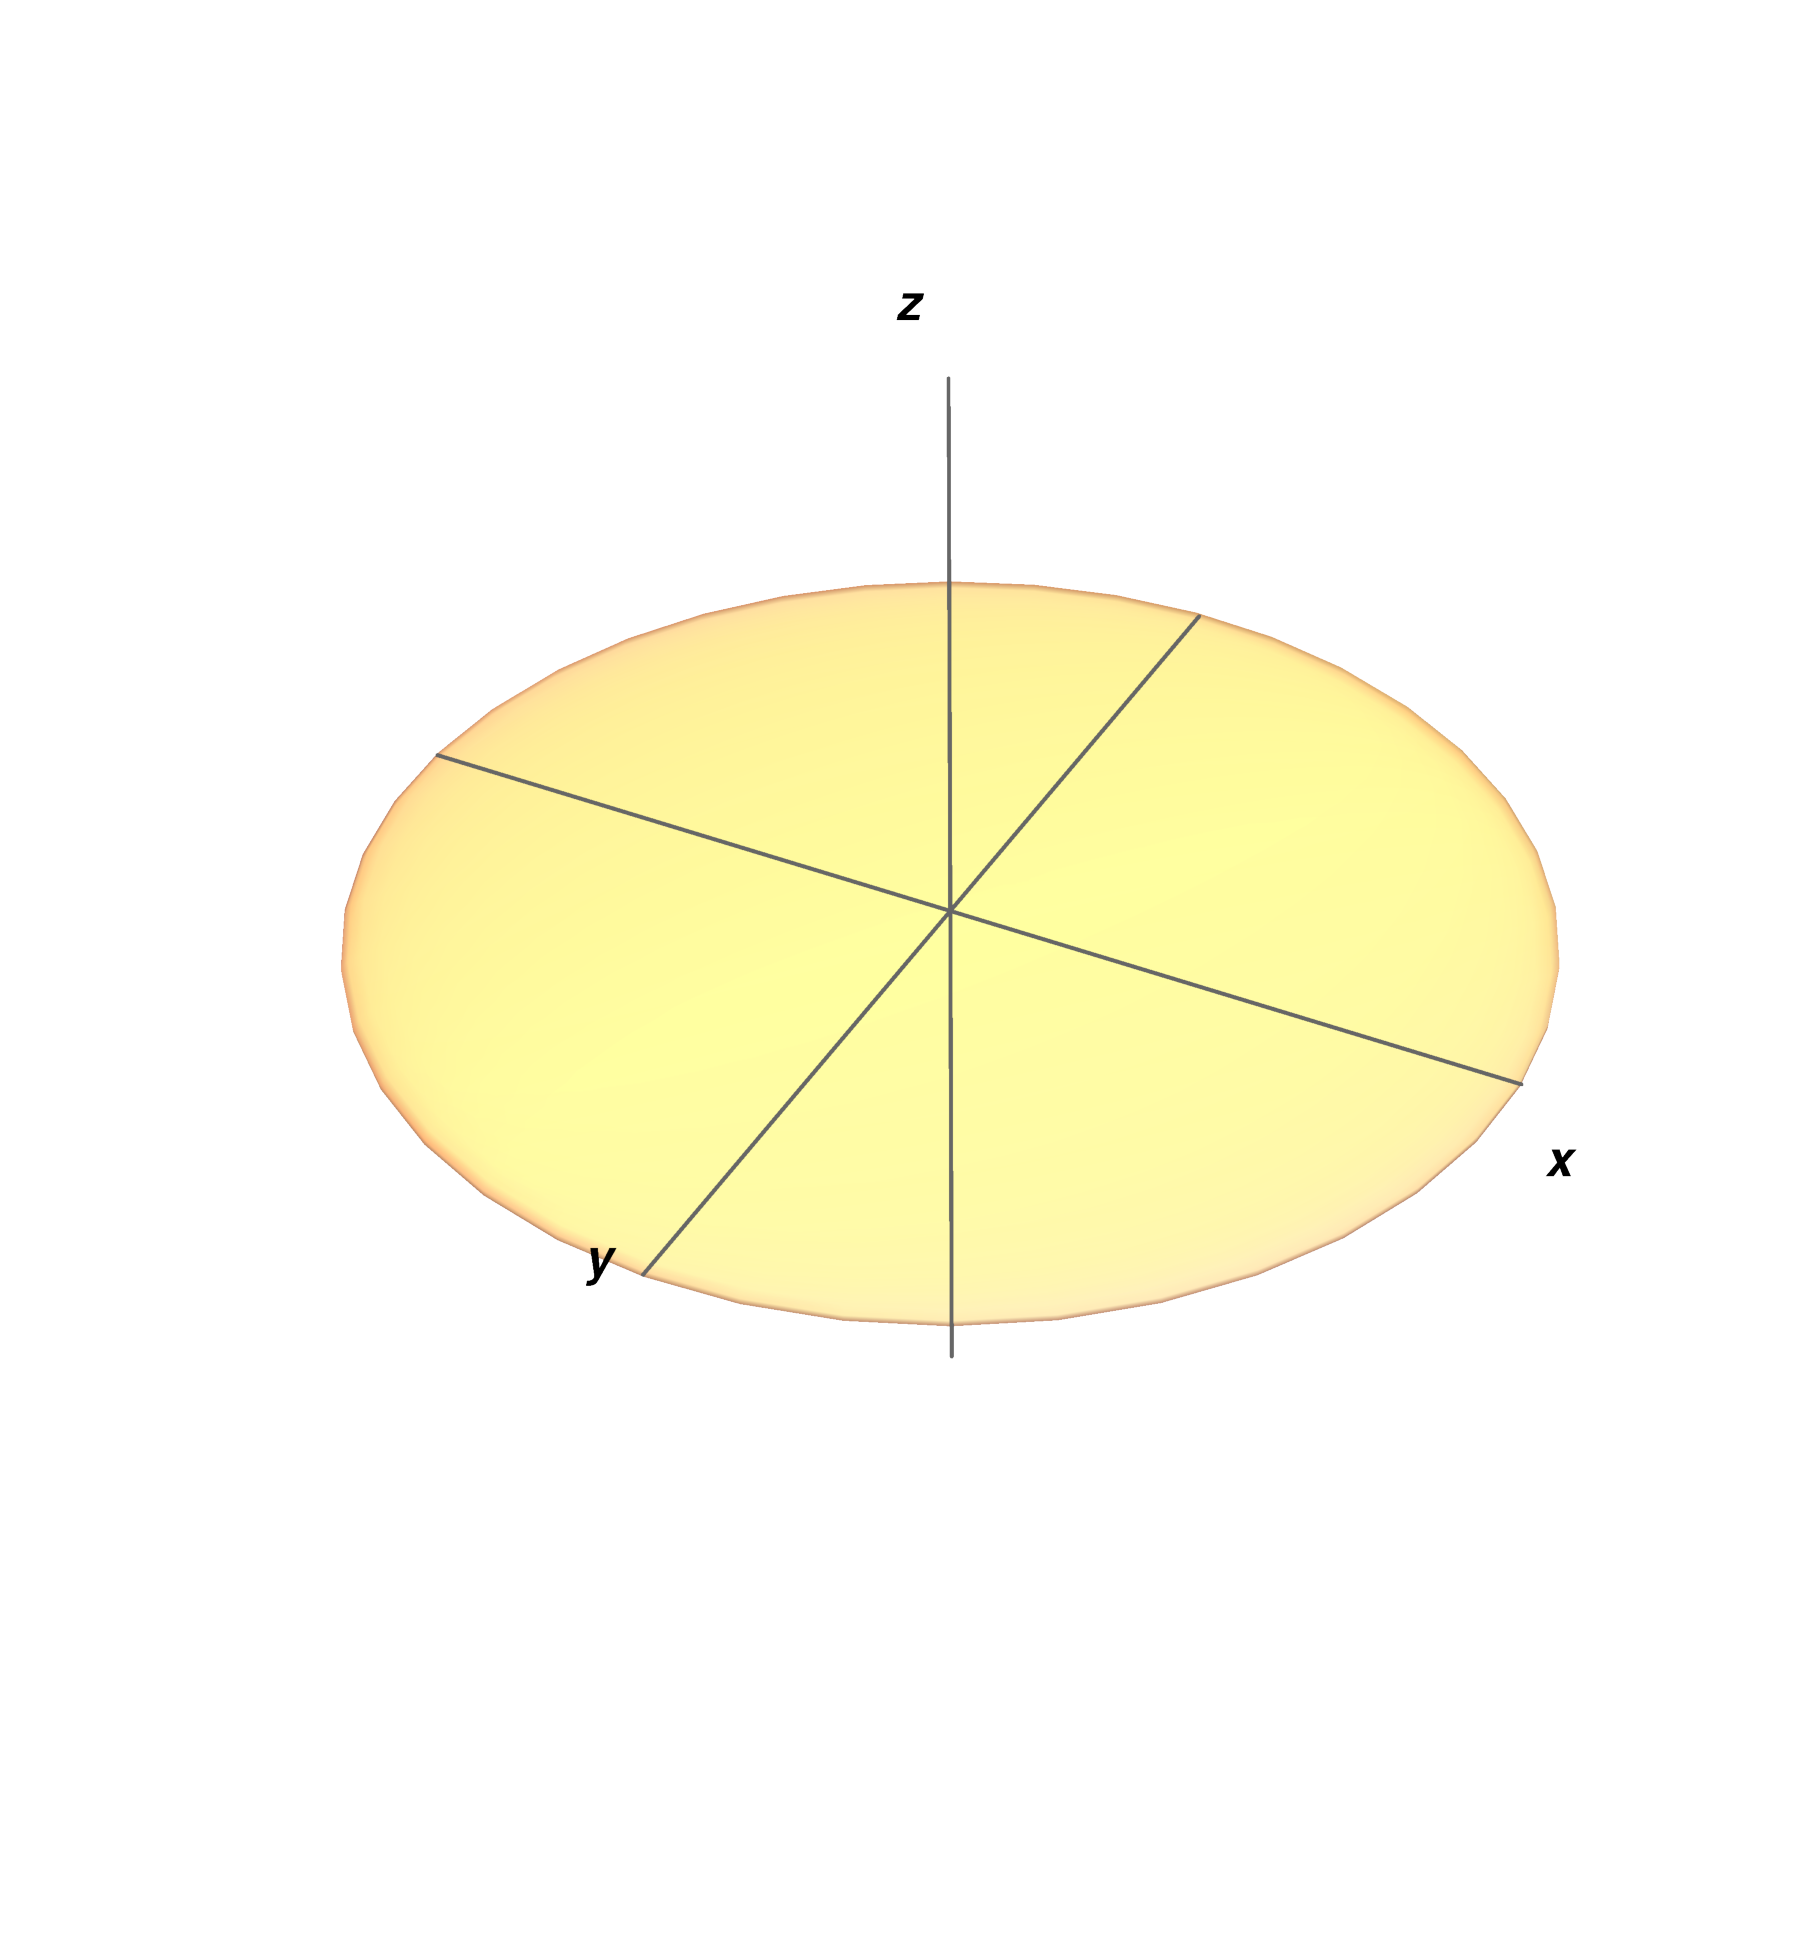
\includegraphics[width=6cm]{DiskXY}
\end{minipage}
\caption{
Deformación de la esfera de Bloch a un disco sobre el plano $XY$.}
\label{fig:qtm-op-motivation}
\end{figure} % }}}
Aunque podemos revisar explícitamente que las propiedades 
de traza unitaria y positividad de $\rho$ en \eqref{eq:rho-1qubit}
se preservan, también podemos argumentar geométricamente
que, dado que el disco final se contiene en la esfera de Bloch, 
las propiedades de la matriz de densidad de 1 qubit se preservan.
Sin embargo, veremos que la acción de $\E_z\ot \1$ 
sobre el estado máximamente entrelazado de 2 qubits 
se transforma en una matriz no positiva.

El estado máximamente entrelazado de 2 qubits es
$\ket{\phi}=\qty(\ket{00}+\ket{11})/\sqrt{2}$~\cite{bengtsson_zyczkowski_2017}.
Ya conocemos cómo transforma $\E_z$ a la matriz de densidad 
escrita en la base de matrices de Pauli será necesario calcular 
la representación de $\dyad{\phi}{\phi}$ en la forma de \eqref{eq:rho-2qubits}
para luego calcular $\E_z\ot \1(\dyad{\phi}{\phi})$.
Las componentes $r_{ij}$ se calculan usando el producto interno
de Hilbert-Schmidt $\Tr\qty(\pauli{i}{j}\dyad{\phi}{\phi})$.
Así encontramos 
\begin{align}
\dyad{\phi}{\phi}=\frac{1}{4}\qty(
\pauli{0}{0}+\pauli{1}{1}-\pauli{2}{2}+\pauli{3}{3}).
\end{align}
\cpnote{Me parece que tienes un problema de normalización}
\janote{Cierto. En esta y en la ecuación 1.24 tenía ese error}
Recordemos que $\E_z$ borra la componente en $r_3$ de la
matriz de densidad de 1 qubit en \eqref{eq:rho-1qubit}. 
Al calcular el superoperador $\E_z\ot  \1$, representación de 
un canal cuántico que veremos en la próxima sección, se encuentra
que la acción de $\E_z\otimes\1$ sobre la matriz de densidad de 2 qubits,
escrita como en \eqref{eq:rho-2qubits}, es borrar 
las componentes de la forma $r_{3j}$,
por consiguiente
\begin{align}
\E_z\otimes\1 \qty(\dyad{\phi}{\phi})=\frac{1}{4}\qty(
\pauli{0}{0}+\pauli{1}{1}-\pauli{2}{2}),
\end{align}
que al calcular su representación matricial se tiene
\begin{align}
\E_z\otimes\1 \qty(\dyad{\phi}{\phi})=
\mqty( 
\frac{1}{4} & 0 & 0 & \frac{1}{2} \\
0 & \frac{1}{4} & 0 & 0 \\
0 & 0 & \frac{1}{4} & 0 \\
\frac{1}{2} & 0 & 0 & \frac{1}{4} \\
).
\end{align}
La matriz  $\E_z\otimes\1\qty(\dyad{\phi}{\phi})$ tiene un 
eigenvalor igual a $-1/4$ y por lo tanto no satisface la condición 
de positividad para ser una matriz de densidad.  
En otras palabras, $\E_z\otimes\1\qty(\dyad{\phi}{\phi})$ 
no representa a un estado físico de 2 qubits.
Se dice que $\E_z$ no es una operación completamente 
positiva porque existen estados en el espacio extendido de 2 qubits para 
el cual la extensión $\E_z\ot \1$ no preserva la positividad del estado. 
Acabamos de mostrar que la condición de completa
positividad surge de la posibilidad que un sistema tiene de encontrarse 
en un estado entrelazado con un \textit{ancilla}.

Ahora vamos a establecer la condición de completa positividad 
de forma precisa. Se dice que una operación $\E$ es CP si 
y sólo si, para cualquier extensión arbitraria de dimensión $K$ 
del espacio de Hilbert $(\hi_N \rightarrow \hi_N \otimes \hi_K)$ 
el operador $\E\otimes\1_K$ es positivo~\cite{bengtsson_zyczkowski_2017}. 
Con esta definición hemos justificado las dos condiciones que 
necesita una operación lineal para ser un canal cuántico.

Un canal cuántico es un mapeo lineal  (1) que preserva las características
de la matriz de densidad y (2) completamente positivo. 
En la literatura se suele utilizar el término operaciones 
completamente positivas que preservan la traza 
(CPTP) para referirse a los canales 
cuánticos~\cite{bengtsson_zyczkowski_2017}. 
En la siguiente y última sección de este capítulo estudiaremos 
algunas representaciones de canales cuánticos. 


%Para escribir a la matriz de densidad utilizaremos 
%la base de productos tensoriales de las matrices de Pauli
%$\{ \sigma_0, \sigma_1, \sigma_2, \sigma_3\}$,
%con $\sigma_0=\1$ y los subíndices $1,2$ y $3$ son nada más 
%una etiqueta $x$, $y$ y $z$, respectivamente.
%Las matrices de densidad para 1 y 2 qubits se 
%escriben como~\cite{nielsen_chuang_2011}
%\begin{align}
%\tilde{\rho}&=\frac{1}{2}\sum_{i=0}^{3} r_i\sigma_i,
%& 
%\tilde{\varrho}&=\frac{1}{4}\sum _{i,j=0, }^{3}r_{ij}\sigma_i\otimes\sigma_j,
%\label{eq:densityMatrices_1and2Qubits}
%\end{align}
%\cpnote{La notacion $\rho^2$ parece un cuadrado. No me gusta la redacción ni la
%nueva notacion. quizá algo como $\rho^{[2]}$ o algo asi}
%
%
%
%donde imponemos que $r_0=r_{00}=1$ para preservar 
%la traza unitaria. Las componentes $r_i$ y $r_{ij}$ son las proyecciones 
%de la matriz de densidad sobre los elementos de la base de productos 
%tensoriales de las matrices de Pauli. En particular para 1 qubit, 
%las componentes $r_x, r_y$ y $r_z$ de $\rho^1$ definen 
%las componentes rectangulares de un punto en la bola \cpnote{Nos refereimos a ella
%normalmente como la esfera de bloch. Sugiero cambiarlo en todas partes} de Bloch.
%La esfera de Bloch es una bola unitaria que se utiliza para 
%representar geométricamente a los estados de 1 qubit
%(ver \Fref{fig:qtm-op-motivation}). De esta manera, con la bola de 
%Bloch tenemos una forma de asociar una representación geométrica 
%con la matriz de densidad de 1 qubit en 
%\eqref{eq:densityMatrices_1and2Qubits}.

%\m Consideremos un sistema 
%total que se compone de un subsistema principal $P$ (el sistema 
%cuántico que nos interesa estudiar) y un subsistema secundario $S$
%(cualquier otro sistema con el que el subsistema principal pueda 
%interaccionar). Nuestro objetivo es estudiar la dinámica de $\rho^P$,
%la matriz de densidad de $P$, y vamos a suponer que el 
%estado de $S$ no lo conocemos \textit{a priori}
%o que sencillamente no nos interesa. La condición de completa positividad
%se hace necesaria de imponer sobre $\E$ cuando consideramos que
%el sistema total podría encontrarse en un estado entrelazado  
%$\rho^{\text{total}}\neq \rho^P\ot\rho^S$\cpnote{aguas}. 
%Esta condición asegura que aún las matrices de densidad
%de estados entrelazados preservarán las propiedades de traza unitaria
%y positividad. 
%
%La acción de $\E_z$ la podemos entender estudiando cómo transforma
%a la matriz de densidad $\rho^1$ en
%\eqref{eq:densityMatrices_1and2Qubits}.
%En términos de las componentes $r_i$ la operación $\E_z$ 
%transforma a $\rho^1$ de la siguiente manera
%\begin{align}
%\qty(1,r_x,r_y,r_z)\mapsto\qty(1,r_x,r_y,0).
%\end{align}
%En la \Fref{fig:qtm-op-motivation} mostramos que $\E_z$ transforma 
%geométricamente a la esfera de Bloch deformándola a un disco
%unitario sobre el plano $x$-$y$. Aunque podemos revisar explícitamente 
%que las propiedades de traza unitaria y positividad de $\rho^1$ 
%se preservan, también podemos argumentar, utilizando la representación
%geométrica, que dado que el disco final se contiene en la esfera de Bloch 
%las propiedades de $\rho^1$ se preservan.
%Sin embargo, veremos a continuación que la acción de $\E_z\ot \1$ 
%sobre el estado máximamente entrelazado de 2 qubits 
%se transforma en una matriz no positiva.
%El estado máximamente entrelazado de 2 qubits es
%$\ket{\phi}=\qty(\ket{00}+\ket{11})/\sqrt{2}$~\cite{bengtsson_zyczkowski_2017}.
%Como conocemos cómo transforma $\E_z$ a la matriz de densidad 
%escrita en la base de Pauli será necesario calcular 
%la representación de $\dyad{\phi}{\phi}$ en esa base para 
%luego calcular $\E_z\ot \1(\dyad{\phi}{\phi})•$.
%Las componentes $r_{ij}$ se calculan usando el producto interno
%de Hilbert-Schmidt $\Tr\qty(\pauli{i}{j}\dyad{\phi}{\phi})$.
%Así encontramos 
%\begin{align}
%\dyad{\phi}{\phi}=
%\pauli{0}{0}+\pauli{1}{1}-\pauli{2}{2}+\pauli{3}{3}.
%\end{align}
%
%Ya que $\E_z$ borra la componente en $r_z$ de $\rho^1$ inferimos 
%que la acción de $\E_z\otimes\1$ sobre $\rho^2$ borra 
%las componentes de la forma $r_{3j}$\cpnote{Esto no me parece obvio. creo que 
%toca argumentarlo un poco mejor. o decir qeu uno lo puede probar usando matrices
%y extensiones.}, por consiguiente
%\begin{align}
%\E_z\otimes\1 \qty(\dyad{\phi}{\phi})=
%\pauli{0}{0}+\pauli{1}{1}-\pauli{2}{2},
%\end{align}
%y en su forma matricial se escribe
%\begin{align}
%\E_z\otimes\1 \qty(\dyad{\phi}{\phi})=
%\mqty( 
%\frac{1}{4} & 0 & 0 & \frac{1}{2} \\
%0 & \frac{1}{4} & 0 & 0 \\
%0 & 0 & \frac{1}{4} & 0 \\
%\frac{1}{2} & 0 & 0 & \frac{1}{4} \\
%).
%\end{align}
%La matriz  $\E_z\otimes\1\qty(\dyad{\phi}{\phi})$ tiene un 
%eigenvalor igual a $-1/4$ y por lo tanto no satisface la condición 
%de positividad para ser una matriz de densidad.  
%En otras palabras, $\E_z\otimes\1\qty(\dyad{\phi}{\phi})$ 
%no representa a un estado físico de 2 qubits.
%Se dice que $\E_z$ no es una operación completamente 
%positiva porque existe un estado en el espacio extendido de 2 qubits para 
%el cual la extensión $\E_z\ot \1$ no es un mapeo afín de 
%matrices de densidad \cpnote{aguas}. Acabamos de mostrar que la condición de completa
%positividad surge de la posibilidad que un sistema tiene de encontrarse 
%en un estado entrelazado con otro sistema secundario\cpnote{A veces nos
%referimos a este sistema como auxiliar o ancilla, quiza en italicas, checa a ver 
%como va}. \m


% }}}
\section{Representaciones de los canales cuánticos} % {{{
\label{sec:qtm-channels-representation}
\esqueleto{Enunciar que existen las representaciones de 
Kraus y de superoperador. Copy-paste de las secciones en las 
que hablamos de las representaciones en el informe final. Planeo
dejar sólo un ejemplo y matar los ejemplos de las dos representaciones
en un tiro.}

Los canales cuánticos pueden representarse como superoperadores
o en la representación de suma de operadores de Kraus. 
La matriz de densidad es un operador que actúa sobre el espacio 
de Hilbert, por consiguiente, la ecuación \eqref{eq:E(rho)} 
sugiere que $\E$ es un operador que actúa sobre el espacio 
de Hilbert-Schmidt (espacio en el que viven las matrices de densidad). 
A esta clase de operadores es a los que se les conoce como 
superoperadores~\cite{preskill1998lecture}.
Por otro lado, la representación de Kraus es una forma de 
representar a un canal cuántico con operadores que pertenecen
al mismo espacio en el que se contienen las matrices de densidad.

Un superoperador actúa sobre la matriz de densidad 
como un vector columna. Por ello, discutiremos un procedimiento 
para `vectorizar' a la matriz de densidad.
Consideremos una matriz de densidad $\hat{\rho}$ de dimensión $d\times d$.
La matriz $\hat{\rho}$ puede escribirse como 
un vector columna $\vec{\rho}$, con $d^2$ elementos, 
ordenando los elementos de matriz según la ecuación  
\begin{align}
\rho_k=\hat{\rho}_{ij}, 
\label{eq:matrix-to-vector}
\end{align}
donde $k=\qty(i-1)d+j$, con $i,j=,1,\ldots,d$. 

Para establecer más adelante una manera de evaluar la CP de una operación 
lineal vamos a introducir a continuación una notación de 4 índices para 
etiquetar a los elementos de matriz de un operador que actúa 
sobre un espacio bipartito y una transformación conocida como 
\textit{reshuffle} para reordenar a una matriz. 
Supongamos que $U$ es un operador 
que actúa sobre un espacio de Hilbert 
$\hi$ de la forma $\hi=\hi_M\otimes\hi_N$.
Consideremos una base ortonormal $\ket{m}$ de $\hi_M$ 
y una base ortonormal $\ket{\mu}$ de $\hi_N$. 
Los productos $\ket{m}\otimes\ket{\mu}$ definen a una base
ortonormal del espacio compuesto $\hi$. 
Nótese el uso de letras latinas para los índices del
primer subsistema y letras griegas para los índices del segundo. 
Un elemento de matriz de $U$ se puede etiquetar como
\begin{align}
U_\ind{m\mu}{n\nu}=\matrixel{m\otimes \mu}{U}{n\otimes \nu}.
\label{eq:4indices}
\end{align}
En esta notación de cuatro índices la transformación de \textit{reshuffle}, 
para reordenar a una matriz  $U$, se define 
como~\cite{bengtsson_zyczkowski_2017}
\begin{align}
U^R_\ind{m\mu}{n\nu} = U_\ind{mn}{\mu\nu}.
\label{eq:R-4ind}
\end{align}
Con esta nueva notación y una definición de 
la transformación de \textit{reshuffle}
contamos con las herramientas necesarias para establecer 
las condiciones que un superoperador $\E$ debe satisfacer 
para ser un canal cuántico.

Un canal cuántico es una operación lineal completamente
positiva que preserva las características de la matriz de densidad.
Es decir, un canal cuántico transforma a la matriz de densidad de
tal manera que preserva su (1) Hermiticidad, (2) traza unitaria y 
(3) positividad semidefinida. Para que esto se satisfaga, un 
canal cuántico $\E$ debe cumplir~\cite{bengtsson_zyczkowski_2017}:
\begin{align}
\txt{(i)}&& \rho'=\qty(\rho')^{\dagger}&&\Leftrightarrow
    && \E_\ind{m\mu}{n\nu}=\E_\ind{\mu m}{\nu n}^*,&&
    \label{eq:H-condition}\\
\txt{(ii)}&&\Tr(\rho')=1
    &&\Leftrightarrow&&  \sum_{m}\E_\ind{mm}{n\nu}=\delta_{n\nu},\\     
\txt{(iii)}&&\rho'\geq0
    &&\Leftrightarrow&&  \sum_{n\nu}\E_{\ind{m\mu}{n\nu}}\rho_{n\nu}\geq0 &
    \text{\hspace{8pt}cuando\hspace{4pt}} \rho>0.
    \label{eq:positivity-condition}
\end{align}
Adicionalmente, para evaluar la completa positividad de $\E$ es 
necesario introducir a la matriz de Choi $D_{\E}$ de un canal cuántico.
La matriz $D_{\E}$ se define como la matriz resultante de 
aplicar la transformación de \textit{reshuffle} al superoperador $\E$,
es decir, $D_{\E}=\E^{R}$~\cite{bengtsson_zyczkowski_2017}.
Finalmente, la condición de CP de $\E$, utilizando a su matriz de Choi, 
está establecida en el siguiente teorema.
\begin{thm}{Teorema de Choi.}\label{thm:choi-CP}
Un superoperador lineal $\E$ es completamente positivo si y sólo si 
su matriz de Choi asociada $D_{\E}$ es positiva semidefinida.
\end{thm}
\begin{proof}
Vamos a presentar la demostración expuesta por Bengtsson
en~\cite[p. 281]{bengtsson_zyczkowski_2017}.
La matriz de Choi $D_{\E}$ de un 
canal cuántico $\E$ es una matriz Hermítica que 
actúa sobre el espacio de Hilbert-Schmidt $\mathcal{H}_{N^2}$
(espacio de las matrices de dimensión $N^2\times N^2$). 
Utilizando el teorema de descomposición 
espectral~\cite{nielsen_chuang_2011},
\begin{align}
D_{\E}&=\sum_{i}\lambda_i\dyad{\chi_i}{\chi_i}
&
D_{\ind{mn}{\mu\nu}}&=\sum_i\lambda_i
\chi^i_{mn}\qty(\chi_{\mu\nu}^i)^*,
\end{align}
donde los eigenvalores $\lambda_i\in\mathbb{R}$. Ahora consideremos
la acción de $\E\ot \1_N$ sobre un estado puro $z_{nn'}z^*_{\nu\nu'}$,
\begin{align}
\rho'_{mm'\mu\mu'}&=
\sum_{n,n',\nu,\nu'}
\E_{\ind{m\mu}{n\nu}}\delta_{\ind{m'\mu'}{n'	\nu'}}z_{nn'}z^*_{\nu\nu'}
=
\sum_{n,\nu}
\E_{\ind{m\mu}{n\nu}}z_{nm'}z^*_{\nu\mu'},
\end{align}
donde $\delta_{\ind{m'\mu'}{n'	\nu'}}=\delta_{m'n'}\delta_{\mu'\nu'}$,
\begin{align}
\sum_{n,\nu}\E_{\ind{m\mu}{n\nu}}z_{nm'}z^*_{\nu\mu'}&=
\sum_{n,\nu}D_{\ind{mn}{\mu\nu}}z_{nm'}z^*_{\nu\mu'}\nonumber\\
\rho'_{mm'\mu\mu'}&=
\sum_{n,\nu,i}\lambda_{i}
\chi^i_{mn}z_{nm'}\qty(\chi_{\mu\nu}^iz_{\nu\mu'})^*,
\end{align}
donde utilizamos $\E_{\ind{m\mu}{n\nu}}
=\E^R_{\ind{mn}{\mu\nu}}
=D_{\ind{mn}{\mu\nu}}$.
Finalmente, para evaluar que $\rho'$ sea una matriz de densidad positiva 
calculamos sus elementos de matriz con un vector arbitrario~$y_{mm'}$
para encontrar la condición que se debe de satisfacer,
\begin{align}
\sum_{m,m',\mu,\mu'}
y_{mm'}\rho'_{mm'\mu\mu'}y_{\mu\mu'}=
\sum_{m,m',n,n'}\lambda_i\abs{
y_{mn'}\chi^i_{mn}z_{nm'}}^2
\geq0,
\end{align}
entonces $\lambda_i\geq1$. Por consiguiente, la matriz 
de Choi $D_{\E}$ debe ser positiva semidefinida para que $\rho'$ 
también lo sea.
\end{proof}
En resumen, las condiciones \eqref{eq:H-condition} 
a \eqref{eq:positivity-condition}, más el teorema \eqref{thm:choi-CP},
establecen las restricciones sobre el superoperador $\E$ para que sea
un canal cuántico~\cite{bengtsson_zyczkowski_2017}.

Por el otro lado, un canal cuántico $\E$ también puede escribirse
en la representación de suma de operadores.
En 1971, Karl Kraus introdujo esta representación como resultado
del teorema de Stinespring \cite{bengtsson_zyczkowski_2017}.
La representación de Kraus de un canal cuántico reescribe
a la ecuación \eqref{eq:E(rho)} como
$\E\qty(\rho)=\sum_k E_k\rho E_k^{\dagger}$,
para algún conjunto de operadores $\{E_k\}$ 
que satisfacen la condición 
$\sum _kE_k^{\dagger}E_k\leq\1$~\cite{nielsen_chuang_2011}. 
Esta representación se relaciona con el superoperador $\E$ por
medio de la matriz de Choi.

La representación de Kraus no es única y, por ello, es de interés
determinar un conjunto $\{E_k\}$ de operadores canónicos de $\E$.
Se puede encontrar un conjunto de operadores canónicos de Kraus de 
un canal cuántico $\E$ a partir de los eigenvectores normalizados 
$\ket{\chi_k}$ de la matriz de Choi reordenados como matrices 
mediante el proceso inverso
establecido en \eqref{eq:matrix-to-vector}~\cite{bengtsson_zyczkowski_2017}.
Además, la raíz cuadrada de los eigenvalores $\sqrt{\lambda_k}$ de 
$D_{\E}$ proporcionan los pesos de los operadores canónicos $E_k$.

\textbf{Forma canónica de Kraus.} Un mapeo completamente 
positivo $\E:\mathcal{M}^{(N)}\to\mathcal{M}^{(N)}$ se
puede escribir como
\begin{align}
\rho \longrightarrow \rho' = 
\sum_{k=1}^{r\leq d^2}\lambda_k\chi_k\rho\chi_k^{\dagger}
= \sum_{i=1}^rE_k\rho E_k^{\dagger},
\label{eq:Kraus-canonical}
\end{align}
donde $r$ es el rango de $D_{\E}$ y $\chi_k$ sus eigenvectores
$\ket{\chi_k}$ reordenados como matrices. Esto quiere decir que 
$E_k=\sqrt{\lambda_k}\chi_k$. Además, los 
operadores $E_k$ deben satisfacer la condición
\begin{align}
  \Tr\qty(E_i^{\dagger}E_j)=d_i\delta_{ij}.
  \label{eq:Tr-Kraus-canonical}
\end{align}
Si canal cuántico $\E$ preserva la $\Tr \rho$, se cumple que
\begin{align}
  \sum_kE_k^{\dagger}E_k=\1
  \hspace{0.5cm}\Rightarrow\hspace{0.5cm}
  \sum_{k=1}^r\lambda_k=N .
  \label{eq:completeness-Kraus-canonical}
\end{align}
Se conoce como rango de Kraus al número de operadores 
en la forma canónica. Es decir, el número de términos en la sumatoria
en \eqref{eq:Kraus-canonical}. Por consiguiente, el rango de 
Kraus de $\E$ es igual al rango de su matriz de Choi 
$D_{\E}$~\cite{bengtsson_zyczkowski_2017}.

Con esto completamos los fundamentos teóricos para estudiar 
el problema de las operaciones PCE a partir del siguiente capítulo. 
Primero presentamos a la matriz de densidad como una herramienta 
para representar a los estados cuánticos. Luego, expusimos la teoría 
de los canales cuánticos para estudiar la dinámica de los sistemas 
cuánticos abiertos. Un canal cuántico es una operación
completamente positiva que preserva las características de la 
matriz de densidad. Ahora nos vamos a centrar en estudiar una 
dinámica muy particular de los sistemas de qubits.
% }}}
%%% Lo que está comentado abajo era parte del modelo, puede ser útil  después  {{{
%%%%%%%%%%%%%%%%%%%%%%%%%%%%%%%%%%%%%%

%En adición a los conjuntos de puntos que se trabajan con normalidad
%en Matemáticas ~---puras y aplicadas---, se tendrá que hacer uso
%frecuentemente de los conjuntos de conjuntos, si por ejemplo $X$ es
%la recta real, como un intervalo es un conjunto de puntos, es decir
%un subconjuto de $X$, se tendrá que el conjunto de todos los
%intervalos es un conjunto de conjuntos.
%
%En especial, cuando una clase hace referencia a subconjuntos del
%conjunto $X$, la llamaremos \textbf{familia}. En especial el
%\textbf{conjunto potencia} $\mathcal{P} (X)=\{A\mid A\subseteq X\}$
%es una familia de $X$. Asimismo, se definirá el \textbf{complemento}
%de $A$ por \[A^c=\{x\mid x\notin A\}.\]
%
%\begin{defn}\label{dfcp28} Una \textbf{función de selección}
%para un conjunto $X$ es una función $f$ la cual asocia a cada
%subconjunto no vacío $E$ de $X$ un elemento de $E$: $f(E)\in E$.
%\end{defn}
%
%\begin{axm}[de selección]\label{choice} Para cualquier conjunto
%existe una función de selección.
%\end{axm}
%
%\begin{rem} Con frecuencia el axioma~\ref{choice} se presenta en
%la forma: para cada $E\in \mathcal{P}(X)\setminus\{\nada\}$,
%elegimos un elemento $x\in E$. Asimismo, es equivalente al lema de
%Zorn, para más detalles consultar
%~\cite[p. 97]{Halmo},~\cite[p. 338]{Haus} o~\cite[p. 14]{Hewit}.
%\end{rem}
%
%Una \textbf{clase disjunta} es una clase {\boldmath $A$} de
%conjuntos tal que para cualquier par de conjuntos distintos de
%{\boldmath $A$} son disjuntos, en este caso nos referiremos a la
%unión de conjuntos de {\boldmath $A$} como \textbf{unión disjunta}.
%
%Si $E$ es un subconjunto de $X$, la función $\chi _E$ definida para
%$x\in X$ por la relación:
%\begin{equation}\label{eq0}
%    \chi_E(x)= \begin{cases}
%    1, & \mbox{si } x\in E, \\
%    0, & \mbox{si } x\notin E.
%    \end{cases}
%\end{equation}Es llamada \textbf{función característica}
%del conjunto $E$. La correspondencia entre los conjuntos y sus
%funciones características es inyectiva, y todas las propiedades de
%conjuntos y operaciones entre conjuntos pueden ser expresadas por
%medio de funciones características. 
%
%%%%	TABLA CORTA, ÚNICAMENTE LLEVA LÍNEAS HORIZONTALES PARA SEPARAR BLOQUES
%
%\begin{table}[ht]
%\caption[título optativo de la tabla]{Propiedades de los espacios $L^p$. Fuente: tomada de \cite[Cap. 3]{Brez}.}\label{tablaLp}
%\centering
%\begin{tabular}{cccc}
%\hline
%Espacio & Reflexivo\footnote{En el sentido topológico.} & Separable & Dual \\ \hline %\hline
%$L^p$, $1<p<\infty$  & Si & Si & $L^q$, $1/p+1/q=1$ \\
%$L^1$ & No & Si & $L^\infty$ \\
%$L^\infty$ & No & No & $L^1 \varsubsetneq (L^\infty)’$ \\ \hline
%\end{tabular}
%\end{table}\footnotetext{En el sentido topológico.} 
%
%\begin{defn}\label{dfcp1}Si $\su En$ es una sucesión de
%conjuntos, definiremos los conjuntos $\overline{\lim } E_n$ y
%$\underline{\lim } E_n$ de la siguiente forma:
%\[\begin{array}{cc}
%  \overline{\lim} E_n=\limsup \limits_{n\rightarrow \infty}E_n =
%  \bigcap \limits_{n=1}^\infty \Union Ein \infty ,&
%  \underline{\lim} E_n=\liminf \limits_{n\rightarrow \infty}E_n =
%  \bigcup \limits_{n=1}^\infty \Inter Ein \infty \\
%\end{array}\] y los llamaremos \textbf{límite superior} y
%\textbf{límite inferior}, respectivamente, de la sucesión $\su En$.
%Si tenemos $\overline{\lim} E_n = \underline{\lim} E_n$, usaremos la
%notación $\lim_n E_n$ para este conjunto. Si la sucesión es tal que
%$E_n\subset E_{n+1},\ n=1,2,\dots$ le llamaremos \textbf{creciente}
%y se denotará por $E_n\!\!\uparrow$ y su límite será $\lim
%\limits_{n\rightarrow \infty}E_n = \union En1 \infty$; si es tal que
%$E_n\supset E_{n+1},\ n=1,2,\dots$ le llamaremos
%\textbf{decreciente} y se denotará por $E_n\!\!\downarrow$ y su
%límite será $\lim \limits_ {n\rightarrow \infty}E_n = \inter En1
%\infty$. En ambos casos nos referiremos a ella como
%\textbf{monótona}.\end{defn}
%
%
%\begin{defn}\label{dfcp2}Sea $f$ una aplicación definida del conjunto
%$X$ al conjunto $Y$, es decir $f:X\To Y$. Para cualquier subconjunto
%$T\subseteq Y$, definimos la \textbf{imagen inversa} de $T$, bajo
%$f$, denotada por $\ff (T)$, como sigue:
%\[\ff (T)=\{s\in X\mid f(s)\in T\}.\]\end{defn} 
%
%\begin{thm}\label{thcp1}Para la aplicación $\ff :{\cal{P}} (Y)
%\To {\cal{P}} (X)$ se tienen las propiedades siguientes:
%\begin{enumerate}
%    \vspace{0pt} \item $\ff(\bigcup_j T_j) = \bigcup_j
%    \ff(T_j)$.
%    \vspace{0pt} \item $\ff(\bigcap_j T_j) = \bigcap_j
%    \ff(T_j)$.
%    \vspace{-6pt} \item Si $T_1\cap T_2=\nada$, entonces
%    $\ff(T_1)\cap \ff(T_2) = \nada$.
%    \vspace{-6pt} \item $\ff(T^c) = [\ff(T)]^c$.
%    \vspace{-6pt} \item $\ff(\nada) = \nada$.
%    \vspace{-6pt} \item $\ff(Y) = X$.
%\end{enumerate}
%\end{thm}
%
%
%Las propiedades (1) y (3) del teorema~\ref{thcp1} establecen las
%condiciones para la unión disjunta en una familia en $Y$. Sea ahora
%$\Df$ una familia cualquiera de subconjuntos de $Y$, y definamos la
%familia $\ff (\Df)$ de subconjuntos de $X$ como
%sigue:\begin{equation}\label{eq1}
%    \ff(\Df) = \{A\subseteq X \mid
%A = \ff(T) \mbox{ para algún } T\in \Df\} = \{\ff(T) \mid T\in
%\Df\}.
%\end{equation}
%
%El sistema de numeros reales extendido o \textbf{recta real
%extendida} es el conjunto definido por $\RR\df\R \cup \{-\infty,
%+\infty\}$, con la siguiente relación de orden: para $a\in \R$
%tenemos $-\infty <a< +\infty$. La topología para este conjunto se
%define por declarar como abiertos a los siguientes conjuntos:
%$(a,b),\ [-\infty,b),\ (a,+\infty]$ y cualquier unión de conjuntos
%de este tipo. Cuando se haga referencia a los \textbf{numeros reales
%extendidos} o \textbf{valor real extendido}, se estará hablando de
%los numeros reales y de los símbolos $\pm\infty$. Cuando trabajamos
%con teoría de la integración, nos encontraremos con $\infty$, una
%razón es que algunas veces trataremos de integrar sobre conjuntos de
%medida infinita, este es caso de la recta real.
%
%Por tal motivo, se hacen las siguientes definiciones para
%facilitar su manejo: $a+\infty = \infty+a \df \infty$ si $0\leq a
%\leq \infty$,~y
%\begin{equation}\label{eq4}
%    a\cdot \infty = \infty \cdot a
%\df\begin{cases}
%  \infty, & \mbox{si } 0 < a \leq \infty \\
%  0, & \mbox{si } a = 0 \\
%\end{cases}
%\end{equation}las leyes de cancelación se tratan
%así: $a+b = a+c\ \Rightarrow\ b=c\ $ y $a\cdot b =a\cdot c\
%\Rightarrow\ b=c$ sólo cuando $0 < a < \infty$. 
%
%\begin{defn}\label{dfcp3}Sea $\su aj$ una sucesión en la recta
%real extendida, y sean $b_k = \sup\{a_k,a_{k+1},a_{k+2}\dots\},\
%k=1,2,3,\dots$, y $\beta = \inf\{b_1,b_2,b_3,\dots\}$. Entonces
%llamaremos a $\beta$ el \textbf{límite superior} de $\su aj$, y
%escribiremos $\beta = \limsup \limits_{j\rightarrow \infty}(a_j)$.
%El \textbf{límite inferior} se define análogamente, al intercambiar
%$\sup$ e $\inf$ en las anteriores definiciones; notemos que \[\liminf
%\limits_{j\rightarrow \infty}(a_j) = -\limsup \limits_{j\rightarrow
%\infty}(-a_j).\] Si $\su aj$ converge, entonces tenemos $\liminf
%\limits_{j\rightarrow \infty}(a_j) = \limsup \limits_{j\rightarrow
%\infty}(a_j) = \lim \limits_{j\rightarrow
%\infty}(a_j)$.\end{defn}
%
%\begin{prp}\label{prcp1}Si $0\leq a_1\leq a_2\leq \cdots$,
%$0\leq b_1\leq b_2\leq \cdots$, tales que $a_j \To a$ y $b_j \To
%b$. Entonces $a_j b_j \To ab$.
%\end{prp}
%
%\begin{defn}\label{dfcp4}Supongamos que $\su fj$ es una sucesión de
%funciones de valor real extendido en un conjunto $X$. Entonces
%$\sup_j f_j$ y $\limsup \limits_{j\rightarrow \infty} f_j$ son las
%funciones definidas en $X$ por:
%\[\left(\sup_j f_j\right)(x)\df \sup_j(f_j(x)),\quad \left(\limsup
%\limits_{j \rightarrow \infty} f_j\right)(x)\df \limsup \limits_{j
%\rightarrow \infty}(f_j(x)).\] Si $f(x)=\lim \limits_{j \rightarrow
%\infty} f_j(x)$, y asumimos que el límite existe para cualquier
%$x\in X$, entonces llamaremos a $f$ el \textbf{límite puntual} de la
%sucesión $\su fj$ y hablaremos de \textbf{convergencia puntual} en
%este contexto.\end{defn}
%
%\begin{figure}[ht]
%\centering
%\label{fig:analisisGraficoModelo3}
%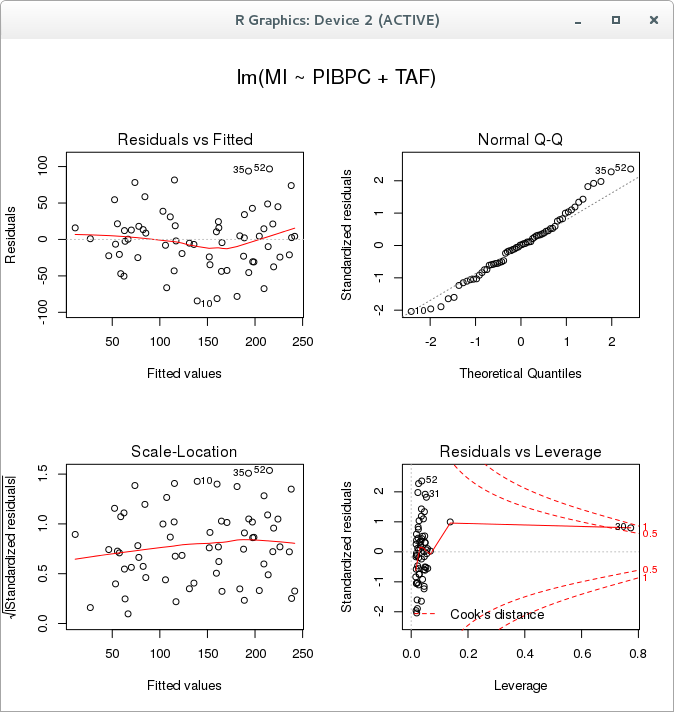
\includegraphics[width=0.9\linewidth]{analisisGraficoModelo3}\\
%\caption[Titulo en el índice de figuras (opcional)]{Título en el 
%documento. Las imágenes pueden ser raster (de preferencia jpg, png 
%con buena resolución para imprimir) o vectorial (convertir a pdf, en 
%este caso la resolución no afecta) Fuente: imagen tomada de~\cite{liu}.}
%\end{figure}
%
%
%\begin{lem}\label{lmcp11}Sean $z,w \in \C$, $1 < p \leq 2$ y $1/p +
%1/q = 1$. Entonces tenemos \[\abs{z+w}^q + \abs{z-w}^q \leq 2 (|z|^p
%+ |w|^p)^{\frac{1}{p-1}}.\]
%\end{lem}
%
%\begin{proof} Consultar~\cite[p. 227]{Hewit}. \end{proof}
%
%\begin{defn}\label{dfcp5}Sea $f:X\To \RR$ una aplicación. Se definen
%las aplicaciones $f^+\!\df\max\{f,0\}$, $f^-\!\df-\min\{f,0\}$, a
%$f^+$ y $f^-$ se les llama la \textbf{parte positiva y negativa} de
%$f$, respectivamente.
%\end{defn}
%
%
%\begin{prp}\label{prcp2}Para cualquier aplicación $f:X\To \R$
%denotaremos su valor absoluto con $\abs f$, entonces tenemos
%\[\abs f=f^++f^-,\quad f=f^+-f^-.\]
%\end{prp}
%
%% --------------->  
%
%\section{Tablas y Gráficas}
%
%Las tablas y gráficas deben tener un título \verb|\caption{text}| que la identifique, debe especificar la \textbf{fuente}, y una etiqueta \verb|\label{text}| para hacer referencias cruzadas dentro del documento.
%
%%% TABLAS LARGAS LLEVAN TODAS LAS DIVISIONES DE LOS BLOQUES
%\subsection{Tablas}
%
%\begin{longtable}{|l|l|l|l|l|}
%\caption[]{Diccionario de datos, tabla \textit{marn} (continuación)} \\ \hline
%
%\multicolumn{1}{|c|}{\textbf{Name}} & \multicolumn{1}{c|}{\textbf{Data type}} & \multicolumn{1}{c|}{\textbf{Not Null?}} & \multicolumn{1}{c|}{\textbf{Primary key?}} & \multicolumn{1}{c|}{\textbf{Default}} \\ \hline \endhead
%	\caption[Diccionario de datos, tabla \textit{marn}]{Diccionario de datos, tabla \textit{marn}. Fuente: obtenida de pgAdminIII}\label{data:marn} \\ \hline
%
%	\multicolumn{1}{|c|}{\textbf{Name}} & \multicolumn{1}{c|}{\textbf{Data type}} & \multicolumn{1}{c|}{\textbf{Not Null?}} & \multicolumn{1}{c|}{\textbf{Primary key?}} & \multicolumn{1}{c|}{\textbf{Default}} \\ \hline \endfirsthead 
%
%	id & \textit{integer} & \textit{Yes} & \textit{Yes} & \textit{nextval('marn\_id\_seq'} \\ %\hline
%
%	 &  &  &  & \textit{::regclass)}\footnote{Note que la tabla es mas ancha que lo preestablecido. Procure diseñar elementos acordes con el espacio preestablecido.} \\ \hline
%
%	\multicolumn{ 5}{|l|}{Clave primaria que  obtendrá su valor de forma secuencial al ingresar un nuevo registro} \\ \hline
%		lista\_tax & \textit{text} & \textit{No} & \textit{No} & \textit{} \\ \hline
%
%	\multicolumn{ 5}{|l|}{Clasificación del proyecto en base al Listado Taxativo del MARN} \\ \hline
%		no\_marn & \textit{text} & \textit{No} & \textit{No} & \textit{} \\ \hline
%
%	\multicolumn{ 5}{|l|}{Numero de expediente asignado por el MARN} \\ \hline
%		date0 & \textit{date} & \textit{No} & \textit{No} & \textit{} \\ \hline
%
%	\multicolumn{ 5}{|l|}{Día del ingreso del expediente del proyecto (instrumento ambiental) en el MARN} \\ \hline
%		notas & \textit{text} & \textit{No} & \textit{No} & \textit{} \\ \hline
%
%	\multicolumn{ 5}{|l|}{Observaciones} \\ \hline
%		no\_res\_ap & \textit{text} & \textit{No} & \textit{No} & \textit{} \\ \hline
%
%	\multicolumn{ 5}{|l|}{Numero de resolución aprobatoria del proyecto por el MARN%
%	\footnote{Note que en esta línea la tabla se corta y continua en la siguiente página. 
%	Utilizar paquete \textsf{longtable} y ambiente \textit{longtable}.}} \\ \hline
%		date\_res\_ap & \textit{date} & \textit{No} & \textit{No} & \textit{} \\ \hline
%
%	\multicolumn{ 5}{|l|}{Día de emisión de la resolución aprobatoria por el MARN} \\ \hline
%		date0\_fianza & \textit{date} & \textit{No} & \textit{No} & \textit{} \\ \hline
%
%	\multicolumn{ 5}{|l|}{Día de emisión de fianza del proyecto.} \\ \hline
%		no\_res\_fianza & \textit{text} & \textit{No} & \textit{No} & \textit{} \\ \hline
%
%	\multicolumn{ 5}{|l|}{Numero de la resolución de aceptación de fianza por el MARN} \\ \hline
%		date1\_fianza & \textit{date} & \textit{No} & \textit{No} & \textit{} \\ \hline
%
%	\multicolumn{ 5}{|l|}{Fecha de inicio de fianza} \\ \hline
%		date2\_fianza & \textit{date} & \textit{No} & \textit{No} & \textit{} \\ \hline
%
%	\multicolumn{ 5}{|l|}{Fecha de finalización de fianza (renovación)} \\ \hline
%		lic\_ambiental & \textit{text} & \textit{No} & \textit{No} & \textit{} \\ \hline
%
%	\multicolumn{ 5}{|l|}{Numero de licencia ambiental} \\ \hline
%		date\_lic\_ambiental & \textit{date} & \textit{No} & \textit{No} & \textit{} \\ \hline
%
%	\multicolumn{ 5}{|l|}{Fecha de finalización de ultima licencia ambiental} \\ \hline
%		proyecto\_id & \textit{integer} & \textit{Yes} & \textit{No} & \textit{} \\ \hline
%
%	\multicolumn{ 5}{|l|}{Enlace con la tabla proyecto\_id} \\ \hline
%\end{longtable}

% }}}


